\newpage
\onecolumn
\centering\textbf{ANNEXES}

\begin{table}[htbp]
    \caption{Communication protocols comparison}
    \begin{center}
    \renewcommand{\arraystretch}{2}
    \begin{tabular}{|p{3cm}|p{4.5cm}|p{4.5cm}|p{4.5cm}|}
    \hline
    \textbf{{Protocols}}& \textbf{\textit{AMQP}}& \textbf{\textit{MQTT}}& \textbf{\textit{HTTP}} \\
    \hline
    Full Name & Advanced Message Queuing Protocol & MQTT (the OASIS standardization group decided it would not stand for anything) & Hyper Text Transfer Protocol\\
    \hline
    Architecture & Queues, multicast (fanout), publish subscribe, request reply & Publish subscribe (MQTT does have a request/reply mode as well) & Request response\\
    \hline
    Command Targets & Exchanges, Queues & Topics & URIs\\
    \hline
    Underlying Protocol & TCP/IP & TCP/IP & TCP/IP\\
    \hline
    Secure connections & TLS + username/password (SASL support possible) & TLS + username/password (SASL support possible) & TLS + username/password (SASL support possible)\\
    \hline
    Client observability & Unknown connection status & Known connection status (will messages) & Unknown connection status\\
    \hline
    Messaging mode & Synchronous and asynchronous & Asynchronous, event-based & Synchronous\\
    \hline
    Messaging queuing & Core capability, flexible configuration & The broker can queue messages for disconnected subscribers & Application needs to implement\\
    \hline
    Message overhead & 8 bytes (general frame format) & 2 bytes minimum (header data can be binary) & 8 bytes minimum (header data is text - compression possible)\\
    \hline
    Message Size & 2GB theoretical, 128MB max recommended & 256MB maximum & No limit but 256MB is beyond normal use cases anyway.\\
    \hline
    Content type & Any (binary) & Any (binary) & Text (Base64 encoding for binary)\\
    \hline
    Topic matching & Level separator: . Wildcards: \* \# & Level separator: / Wildcards: + \# & - \\
    \hline
    Reliability & Two qualities of service: -without acks (=0) - with acks (=1) & Three qualities of service: 0 - fire and forget 1 - at least once 2 - once and only once & Has to be implemented in the application\\
    \hline
    Connection "multiplexing" & Yes - channels & No & -\\
    \hline
    Message attributes & Yes & MQTT 5.0 only & -\\
    \hline
    Object persistence & Yes & Yes & -\\
    \hline
    \end{tabular}
    \label{edge-cloud protocols}
    \end{center}
    \end{table}
    
    
\begin{figure}[!ht]
    \centering
    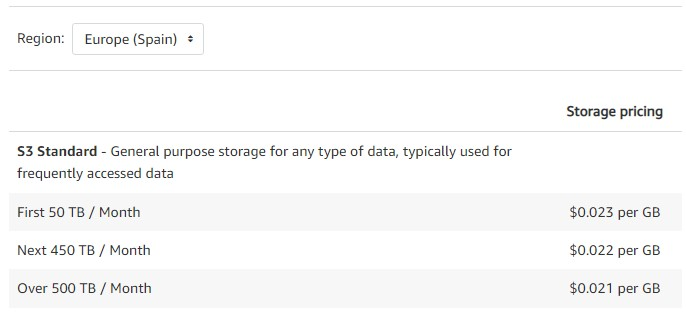
\includegraphics[width=15cm]{functional_performance_specification/images/AWSpricing.jpg}
    \caption{AWS cloud S3 Standard pricing}
    \label{fig:AWS pricing}
\end{figure}